\chapter{Experiments}

    This chapter contains three parts. The first part will show how much compilation time our approach will increase. The second part will show the evaluations of image processing processes' total execution time comparison. The last part will show the evaluations of image processing processes' kernel execution time comparison, including doing kernel fusion by Halide schedule “compute\_at” and our “enqueue\_kernel" approach. Device and other environment informations are listed in table~\ref{tab:my_tab_device}. The benchmark using are blur1D and blur2D. Blur1D means to calculate sum of three pixels, divide it by three and then store the result back. Blur2D means to calculate sum of nine pixels, divide it by nine and then store the result back.

\begin{table}[]
\centering
\caption{Experiment Environment}
\label{tab:my_tab_device}
\begin{tabular}{lllllll}
       & CPU     & frequency & RAM     & compiler   & runtime & runtime version \\
Device & i5-4590 & 3.3GHz    & 8G DDR3 & GCC, Clang & POCL    & v0.11          
\end{tabular}
\end{table}

\section{compilation time increase}
    We normalize compilation time to OpenCL without pre-parser shown in figure~\ref{fig:my_label_ex_1}. The compilation time includes time of OpenCL host API clCreateProgramWithSource. We can see that our pre-parser does not effect the compilation time much.

\begin{figure}[hbtp]
\centering
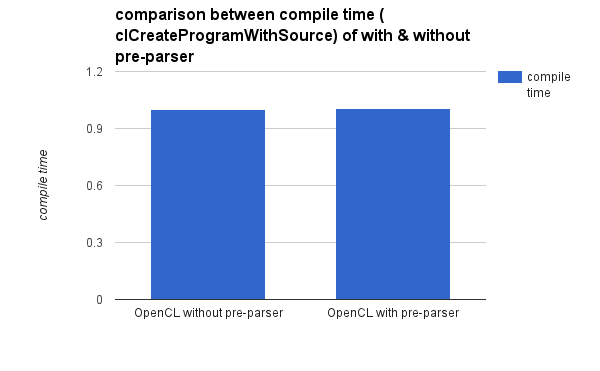
\includegraphics[width=14cm]{img/compile-time.png}
\caption{compilation time comparison between with \& without pre-parser}
\label{fig:my_label_ex_1}
\end{figure}

\section{total execution time comparison}
    We normalize total execution time to OpenCL with kernel fusion shown in figure~\ref{fig:my_label_ex_2}. Since the benefit we can gain by doing kernel fusion will be a constant (OpenCL host APIs overhead), our speedup will decrease as the kernel execution time increase. The total execution time here includes whole OpenCL execution time except compilation time (clCreateProgramWithSource.)
    
\begin{figure}[hbtp]
\centering
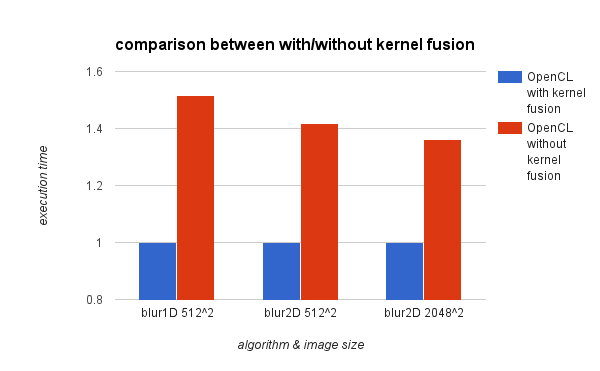
\includegraphics[width=14cm]{img/with-without-2ker.png}
\caption{total execution time comparison between OpenCL with \& without kernel fusion, fusing two kernels into one kernel}
\label{fig:my_label_ex_2}
\end{figure}

\section{kernel execution time comparison}
    We normalize kernel execution time to OpenCL without kernel fusion shown in figure~\ref{fig:my_label_ex_3}. The kernel execution time only includes the time of clEnqueueNDRangeKernel. We set a clWaitForEvents call to wait for the execution event to return and then get the execution time by clGetProfilingInfo. From this figure, we can see that our approach does not have big impact to the kernel execution time.
    
\begin{figure}[hbtp]
\centering
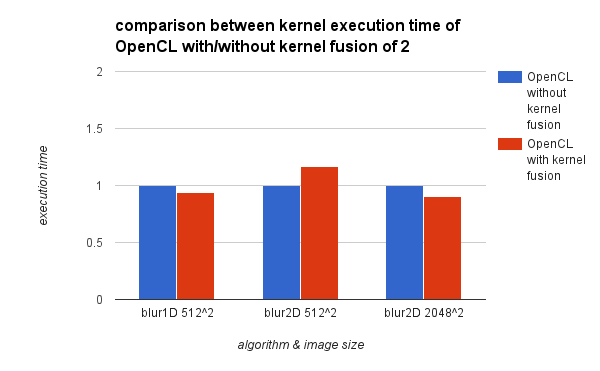
\includegraphics[width=14cm]{img/OpenCL-with-without-execute-2ker.png}
\caption{kernel execution time comparison between OpenCL with \& without kernel fusion, fusing two kernels into one kernel}
\label{fig:my_label_ex_3}
\end{figure}

    We normalize kernel execution time to Halide without kernel fusion shown in figure~\ref{fig:my_label_ex_4}. We can see that the execution time increases as the image kernel size increases or the image size increases.

\begin{figure}[hbtp]
\centering
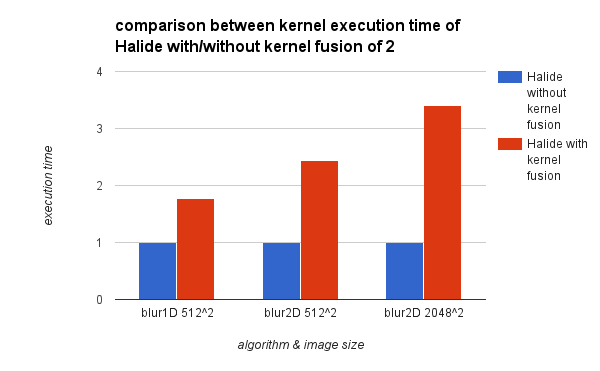
\includegraphics[width=14cm]{img/Halide-with-without-execute-2ker.png}
\caption{kernel execution time comparison between Halide with \& without kernel fusion, fusing two kernels into one kernel}
\label{fig:my_label_ex_4}
\end{figure}

    We normalize kernel execution time to Halide OpenCL CodeGen shown in figure~\ref{fig:my_label_ex_5}. We can see that the kernel execution time of Halide OpenCL CodeGen and our handwritten OpenCL source code are approximately equal. We believe that our handwritten OpenCL source code will do approximately equal operations to Halide OpenCL CodeGen.

\begin{figure}[hbtp]
\centering
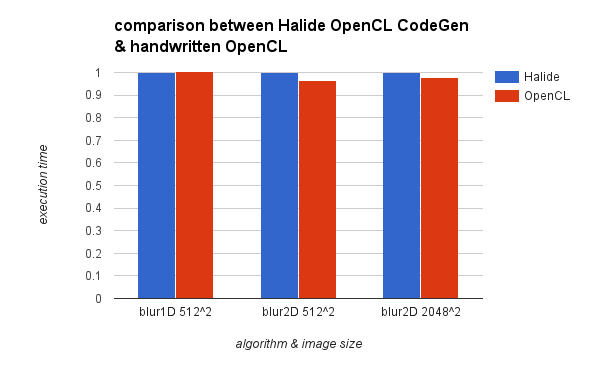
\includegraphics[width=14cm]{img/Halide-OpenCL-1ker-comp.png}
\caption{kernel execution time comparison between Halide OpenCL CodeGen \& handwritten OpenCL code, executing single kernel}
\label{fig:my_label_ex_5}
\end{figure}

    We normalize kernel execution time to our handwritten OpenCL source code shown in figure~\ref{fig:my_label_ex_6}. We can see the performances applying our approach are better than the ones applying Halide kernel fusion. These performance differences are due to the redundant works, which increase as the image kernel size increase or image size increase.

\begin{figure}[hbtp]
\centering
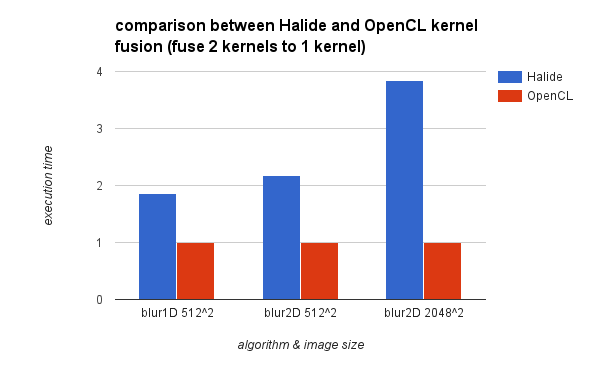
\includegraphics[width=14cm]{img/Halide-OpenCL-2ker-comp.png}
\caption{kernel execution time comparison between Halide \& OpenCL kernel fusion, fusing two kernels into one kernel}
\label{fig:my_label_ex_6}
\end{figure}
